% Packages

\documentclass{beamer}
\setcounter{tocdepth}{1}
\usepackage{graphicx}
\usepackage[export]{adjustbox}
\graphicspath{{Images/}{./}} % Specifies where to look for included images (trailing slash required)
\usepackage{tikz}

\usepackage{booktabs} % Allows the use of \toprule, \midrule and \bottomrule for better rules in tables
\usepackage{pgfplots}
\usepackage{tikz}
\pgfplotsset{width=6cm, compat=newest, every tick label/.append style={scale=0.5}}
\newcommand{\blank}{\begin{frame}\end{frame}}
% Theme
\usetheme{Madrid}

% Font
\usefonttheme{serif}
\usepackage{newtxtext,newtxmath}
\usepackage[default]{lato}

% Inner theme
\useinnertheme{circles}

% Information
\title{Review: Linear equations}
\author{Kin Hei Wong}
\date{\today}
%%%%%%%%%%%%%%%%%%%%%%%%%%%%%%%%%%%%%%%%%%%%%%%%%%%%%%%%%%
\begin{document}

% Title slide
\begin{frame}
    \titlepage
\end{frame}

% Table of Content
\begin{frame}
    \frametitle{Presentation overview}
    \tableofcontents
\end{frame}
%%%%%%%%%%%%%%%%%%%%%%%%%%%%%%%%%%%%%%%%%%%%%%%%%%%%%%%%%%%
% Body slides

\section{1A - Linear equations}
\begin{frame}
    \frametitle{1A}
    \begin{center}
        \title{Linear equations}
        \maketitle
    \end{center}
\end{frame}

\begin{frame}[t]
    \frametitle{Solving linear equations}
    Linear equation is a particular type of equation that comes with one unknown, and first power of variable.\\
    E.g. $3x - 5 = 11$
    \begin{block}{Example 1}
        Solve the equation $3x + 4 = 16$ for $x$.
    \end{block}

    \begin{block}{Example 2}
        Solve $4x + 3 = 3x - 5$.
    \end{block}

    \begin{block}{Example 3}
        Solve $3(2x+5) = 27$.
    \end{block}
\end{frame}

\begin{frame}[t]
    \frametitle{Fractions incoming!}
    \begin{block}{Example 4}
        Solve $\frac{x}{5} - 2 = \frac{x}{3}$.
    \end{block}

    \begin{block}{Example 5}
        Solve $\frac{x-3}{2} - \frac{2x-4}{3} = 5$.
    \end{block}
\end{frame}
\blank


\begin{frame}[t]
    \frametitle{Literal equations}
    Literal equation is just \textbf{Literally algebras only}. However, except for the variable (E.g. $x$), all others are treated as coefficient.\\
    \begin{block}{Example 6}
        Solve $ax + b = cx + d$ for $x$.
    \end{block}
\end{frame}

\begin{frame}
    \frametitle{Exercise 1A}
\end{frame}

%%%%%%%%%%%%%%%%%%%%%%%%%%%%%%%%%%%%%%%%%%%%%%%%%%%%%%%%%%%

\section{1B - Constructing linear equations}
\begin{frame}
    \frametitle{1B}
    \begin{center}
        \title{Constructing linear equations}
        \maketitle
    \end{center}
\end{frame}

\begin{frame}[t]
    \frametitle{Word to equations}
    In this section, we will learn to translate the word problems into algebras and/or equations\\
    \begin{block}{Example 7}
    A chef uses the following rule for cooking a turkey:\\
    'Allow 30 minutes for each kilogram weight of turkey and then add an extra 15 minutes.'
    If the chef forgot to weigh a turkey before cooking it, but knew that it had taken 3 hours to
    cook, calculate how much it weighed.
    \end{block}
\end{frame}

\begin{frame}[t]
    \frametitle{Word to equations 2}
    \begin{block}{Example 8}
        Find the area of a rectangle whose perimeter is $1.08 m$, if it is $8 cm$ longer than it is wide.
    \end{block}
\end{frame}

\begin{frame}[t]
    \frametitle{Word to equations 3}
    \begin{block}{Example 9}
        Adam normally takes 5 hours to travel between Higett and Logett. One day he increases
 his speed by $4 km/h$ and finds the journey from Higett to Logett takes half an hour less
 than the normal time. Find his normal speed.
    \end{block}
\end{frame}

\begin{frame}
    \frametitle{Exercise 1B}
\end{frame}

%%%%%%%%%%%%%%%%%%%%%%%%%%%%%%%%%%%%%%%%%%%%%%%%%%%%%%%%%%%

\section{1C - Simultaneous equations}
\begin{frame}
    \frametitle{1C}
    \begin{center}
        \title{Simultaneous equations}
        \maketitle
    \end{center}
\end{frame}

\begin{frame}[t]
    \frametitle{What is simultaneous equations?}
    Simultaneous means things are happening at the same time. Hence, equations wise, we say it as two equations are 
    drawn or on the graph. But how do we solve the equation? Try drawing the equation for $2x-y=4$ and $x + 2y = 3$. 
    On the graph, if they intersect, it is the solution!
\end{frame}

\begin{frame}[t]
    \frametitle{Substitution vs elimination}
    \begin{block}{Example 10}
        Solve the equations $2x - y = 4$ and $x + 2y = -3$
    \end{block}
\end{frame}

\begin{frame}
    \frametitle{Other simultaneous equations and geometry}
    Are there any simultations equations that no results in 1 solution? YES!!
    \begin{center}
        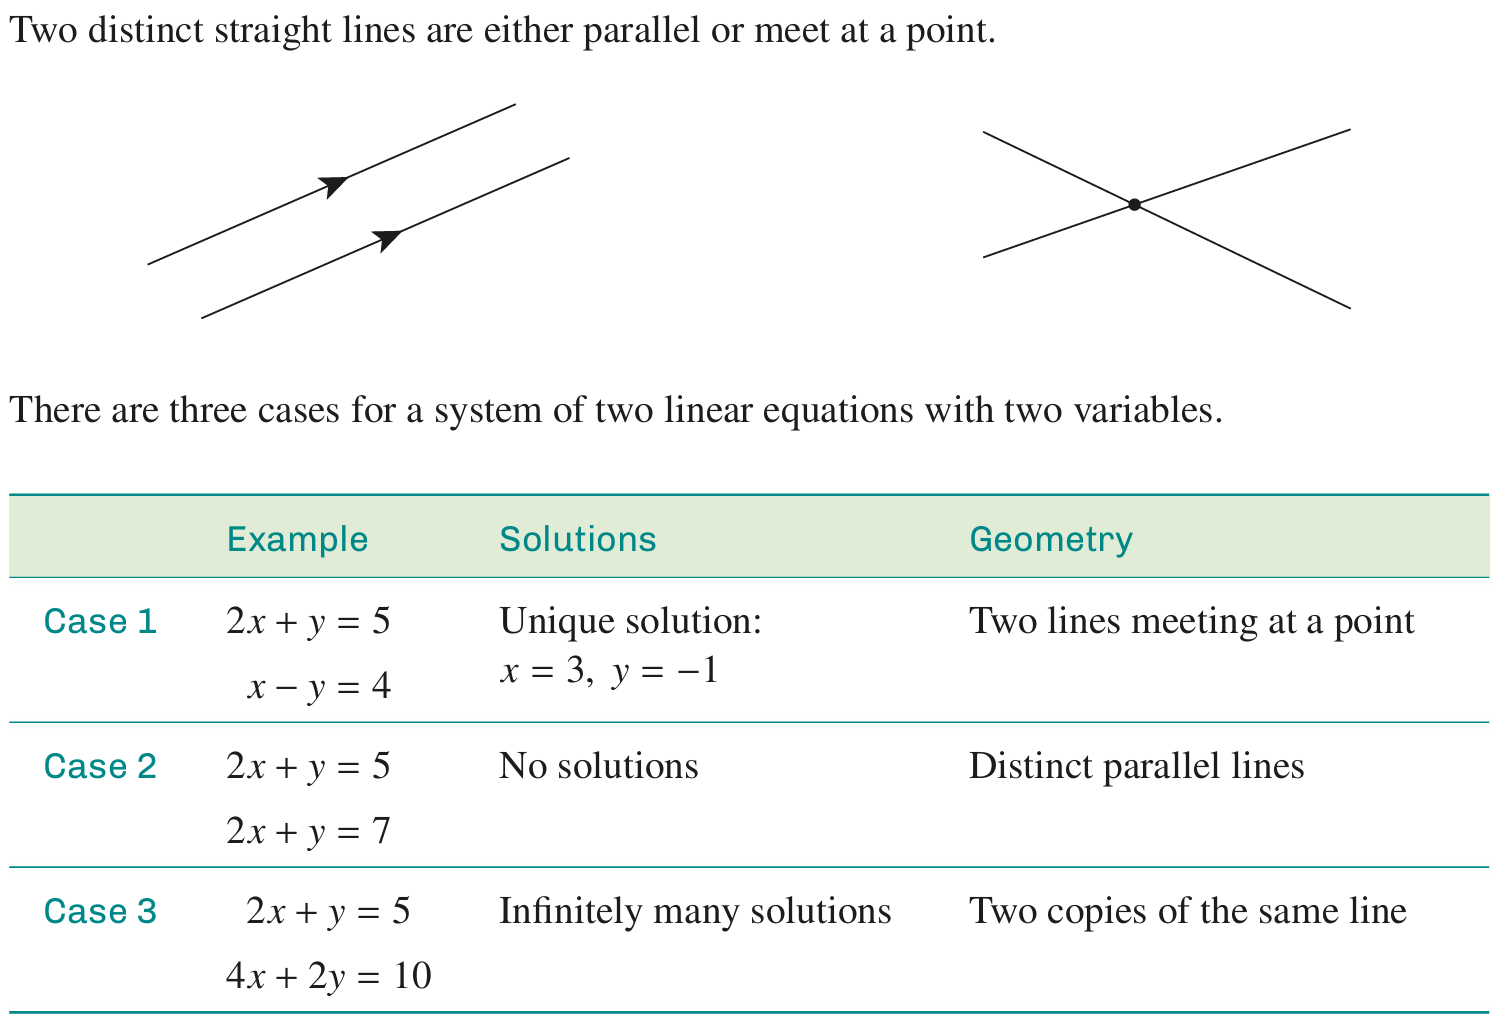
\includegraphics[width = 9.5cm]{Geometry.png}
    \end{center}
\end{frame}

\begin{frame}
    \frametitle{Exercise 1C}
\end{frame}

%%%%%%%%%%%%%%%%%%%%%%%%%%%%%%%%%%%%%%%%%%%%%%%%%%%%%%%%%%%

\section{1D - Constructing simultaneous equations}
\begin{frame}
    \frametitle{1D}
    \begin{center}
        \title{Constructing simultaneous equations}
        \maketitle
    \end{center}
\end{frame}

\begin{frame}[t]
    \frametitle{Making it alive - again...}
    \begin{block}{Example 11}
        The sum of two numbers is 24 and their difference is 96. Find the two numbers.
    \end{block}
\end{frame}

\begin{frame}[t]
    \frametitle{Making it alive - again 2...}
    \begin{block}{Example 11}
        3 kg of jam and 2 kg of butter cost $\$29$, and 6 kg of jam and 3 kg of butter cost $\$54$.
        Find the cost per kilogram of jam and butter.
    \end{block}
\end{frame}

\begin{frame}
    \frametitle{Exercise 1D}
\end{frame}

%%%%%%%%%%%%%%%%%%%%%%%%%%%%%%%%%%%%%%%%%%%%%%%%%%%%%%%%%%%

\section{1E - Solving linear inequalities}
\begin{frame}
    \frametitle{1E}
    \begin{center}
        \title{Solving linear inequalities}
        \maketitle
    \end{center}
\end{frame}

\begin{frame}
    \frametitle{Linear inequalities}
    Inequalities is basically opposite to only 1 answer. Hence, we denote with $\geq, \leq, >, <$. For advanced, 
    we often use $\neq$ in Maths
    \begin{block}{Advanced}
        Proof that 1 + 1 $\neq$ 3.
        \begin{center}
            
\includegraphics[width = 3cm]{Worry.png}
        \end{center}
    \end{block}
    [Don't worry, you won't learn this]
\end{frame}

\begin{frame}[t]
    \frametitle{Swamp of examples incoming}
    \begin{block}{Example 13}
        Solve the inequality $2x + 1 <4$
    \end{block}
    \begin{block}{Example 14}
        Solve the inequality $3 -2x \leq 4$
    \end{block}
    \begin{block}{Example 15}
        Solve the inequality $\frac{2x+3}{5} > \frac{3-4x}{3} +2$
    \end{block}
\end{frame}
\begin{frame}
\end{frame}

\begin{frame}
    \frametitle{Exercise 1E}
\end{frame}

%%%%%%%%%%%%%%%%%%%%%%%%%%%%%%%%%%%%%%%%%%%%%%%%%%%%%%%%%%%

\section{1F - Using and tranposing formula}
\begin{frame}
    \frametitle{1F}
    \begin{center}
        \title{Using and tranposing formula}
        \maketitle
    \end{center}
\end{frame}

\begin{frame}[t]
    \frametitle{They give you formula - We use/rearrange the formula}
    The most common formula we have is A = length $\times$ width. The formula represents as: $A = lw$
    \begin{block}{Example 16}
        Find the area of a rectangle with length ($l$) 10 cm and width ($w$) 4 cm.
    \end{block}
    \begin{block}{Example 17}
        Transpose the formula $v = u + at$ to make a the subject.
    \end{block}
    \begin{block}{Example 18}
        Evaluate $p$ if $2(p + q)-r = z$, and $q = 2$, $r = 3$ and $z = 11$.
    \end{block}
\end{frame}

\begin{frame}[t]
    \frametitle{More applications!}
    \begin{block}{Example 19}
        A path $x$ metres wide surrounds a rectangular lawn. The lawn is $l$ metres long and $b$ metres wide. The total area of the path is A $m^2$.
        \begin{enumerate}
            \item Find A in terms of $l, b$ and $x$.
            \item Find b in terms of $l, A$ and $x$.
            \item Find the value of $b$ if $l = 6, A = 72$ and $x = 1.5$.
        \end{enumerate}
    \end{block}
\end{frame}

\begin{frame}
    \frametitle{More rearrangement}
    \begin{block}{Example 20}
        For each of the following, make c the subject of the formula:\\
        \begin{enumerate}
            \item $e = \sqrt{3c-7a}$
            \item $\frac{1}{a} - \frac{1}{b} = \frac{1}{c-2}$
        \end{enumerate}
    \end{block}
\end{frame}

\begin{frame}
    \frametitle{Exercise 1F}
\end{frame}
\end{document}